\section{Satisfaction Evaluation} \label{sec:satisfationevaluation}

To test how the implemented methods performed compared to each other, the setup from Section \ref{sec:evaluationsetup} was used. Be aware that the scales of the figures differ a bit due to the random selection performing much worse than the other approaches thus dragging the lower end of the scale down.

Figure \ref{fig:testresult4members} presents the average satisfaction when the groups consists of 4 random members. Here there is only little difference in the fond satisfaction with BEC edging out slightly ahead, being a little less than 1\% point better than BC. BTC and BWC are both minimally worse than BC, but as both the methods are more reliant on items being present in multiple top-k lists amongst the users, it is no surprise that they give worse results than BC.

Already when the group size is increased to 8, as seen in Figure \ref{fig:testresult8members}, a trend of BTC outperforming the other methods start emerging, and at 8 members it outperforms BC by about 1.5\% points. An interesting thing to note is that there is a generally sharp drop off in satisfaction for all methods when going from 4 to 8 members, but as the group size is increased, all but BTC drop further, while BTC maintains a satisfaction of around 0.59 until the group size is increased to 40.

\begin{figure}[h]
\centering
\begin{minipage}{.46\textwidth}\centering
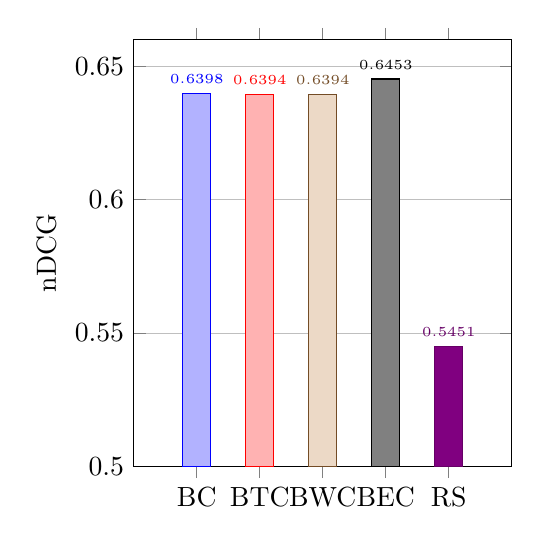
\begin{tikzpicture}
 \begin{axis}[
 	height=7cm,
 	ybar =-10pt,
 	x = .8cm,
 	ymin=0.50, 
 	ymax=0.66,
 	ytick = {0.50,0.55,...,0.70},
 	scaled y ticks = false,
	enlarge x limits ={abs=.8cm},
	nodes near coords,
    every node near coord/.append style={font=\tiny,/pgf/number format/.cd,precision=4},
 	ylabel={nDCG},
	xtick={0,1,2,3,4},  % NEW BIT
	xticklabels={BC, BTC, BWC, BEC, RS},
	%legend style={at={(0.5,-0.1)},
	%anchor=north,legend columns=-1},
	ymajorgrids = true,]

		\addplot coordinates {(0,0.6398)};    
		\addplot coordinates {(1,0.6394)};    
		\addplot coordinates {(2,0.6394)};    
		\addplot coordinates {(3,0.6453)};    
		\addplot coordinates {(4,0.5451)};
        %\legend{BC, BTC, BWC, BEC, Random}
     \end{axis}
\end{tikzpicture}
\captionof{figure}{Groups with 4 users}
\label{fig:testresult4members}
\end{minipage}
\begin{minipage}{.46\textwidth}\centering
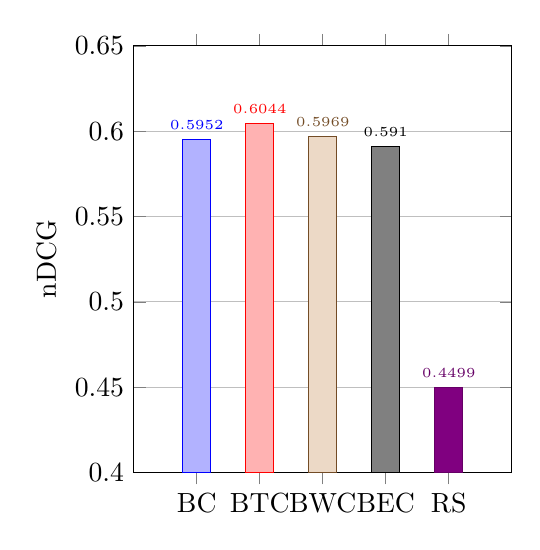
\begin{tikzpicture}
 \begin{axis}[
 	height=7cm,
 	ybar =-10pt,
 	x = .8cm,
 	ymin=0.40, 	
 	ymax=0.65,
 	ytick = {0.40,0.45,...,0.70},
	enlarge x limits ={abs=.8cm},
	nodes near coords,
    every node near coord/.append style={font=\tiny,/pgf/number format/.cd,precision=4},
 	ylabel={nDCG},
	xtick={0,1,2,3,4},  % NEW BIT
	xticklabels={BC, BTC, BWC, BEC, RS},
	%legend style={at={(0.5,-0.1)},
	%anchor=north,legend columns=-1},
	ymajorgrids = true,]

		\addplot coordinates {(0,0.5952)};    
		\addplot coordinates {(1,0.6044)};    
		\addplot coordinates {(2,0.5969)};    
		\addplot coordinates {(3,0.5910)};    
		\addplot coordinates {(4,0.4499)};
        %\legend{BC, BTC, BWC, BEC, Random}
     \end{axis}
\end{tikzpicture}
\captionof{figure}{Groups with 8 users}
\label{fig:testresult8members}
\end{minipage}
\end{figure}

BTC ability to satisfy larger groups becomes truly apparent with a group size of 12 and 16, Figure \ref{fig:testresult12members} and Figure \ref{fig:testresult16members}, where it is about 6.4\% points and 11.2\% points better respectively. An interesting observation is that BTC gives a slightly worse satisfaction with a size of 12 than when the size is 16. The cause of this dip in satisfaction is unknown, however it could be interesting to explore it further. BC, BWC, and BEC all perform within 1\% point of each other, with BEC performing slightly worse than the other two.

When the group size reaches 20, Figure \ref{fig:testresult20members}, BTC also outperforms the other methods the most, at least with the group sizes tested. On average it outperforms BC by about 13.1\% points. However after size 20, the benefits of BTC seems to stagnate, as Figure \ref{fig:testresult40members} shows, at a group size of 40 BTC had a slightly larger fall than the other methods, performing 12.9\% points better than BC.

\begin{figure}[h]
\centering
\begin{minipage}{.46\textwidth}\centering
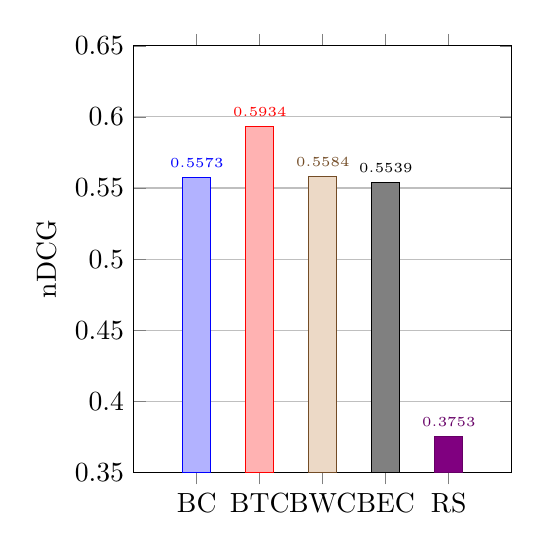
\begin{tikzpicture}
 \begin{axis}[
 	height=7cm,
 	ybar =-10pt,
 	x = .8cm,
 	ymin=0.35, 	
 	ymax=0.65,
 	ytick = {0.35,0.40,...,0.70},
	enlarge x limits ={abs=.8cm},
	nodes near coords,
    every node near coord/.append style={font=\tiny,/pgf/number format/.cd,precision=4},
 	ylabel={nDCG},
	xtick={0,1,2,3,4},  % NEW BIT
	xticklabels={BC, BTC, BWC, BEC, RS},
	%legend style={at={(0.5,-0.1)},
	%anchor=north,legend columns=-1},
	ymajorgrids = true,]

		\addplot coordinates {(0,0.5573)};    
		\addplot coordinates {(1,0.5934)};    
		\addplot coordinates {(2,0.5584)};    
		\addplot coordinates {(3,0.5539)};    
		\addplot coordinates {(4,0.3753)};
        %\legend{BC, BTC, BWC, BEC, Random}
     \end{axis}
\end{tikzpicture}
\captionof{figure}{Groups with 12 users}
\label{fig:testresult12members}
\end{minipage}
\begin{minipage}{.46\textwidth}\centering
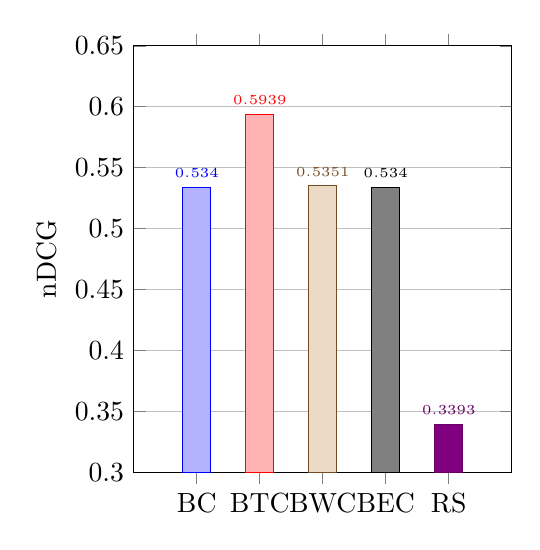
\begin{tikzpicture}
 \begin{axis}[
 	height=7cm,
 	ybar =-10pt,
 	x = .8cm,
 	ymin=0.30, 	
 	ymax=0.65,
 	ytick = {0.30,0.35,...,0.70},
	enlarge x limits ={abs=.8cm},
	nodes near coords,
    every node near coord/.append style={font=\tiny,/pgf/number format/.cd,precision=4},
 	ylabel={nDCG},
	xtick={0,1,2,3,4},  % NEW BIT
	xticklabels={BC, BTC, BWC, BEC, RS},
	%legend style={at={(0.5,-0.1)},
	%anchor=north,legend columns=-1},
	ymajorgrids = true,]

		\addplot coordinates {(0,0.5340)};    
		\addplot coordinates {(1,0.5939)};    
		\addplot coordinates {(2,0.5351)};    
		\addplot coordinates {(3,0.5340)};    
		\addplot coordinates {(4,0.3393)};
        %\legend{BC, BTC, BWC, BEC, Random}
     \end{axis}
\end{tikzpicture}
\captionof{figure}{Groups with 16 users}
\label{fig:testresult16members}
\end{minipage}
\end{figure}



\begin{figure}[h]
\centering
\begin{minipage}{.46\textwidth}\centering
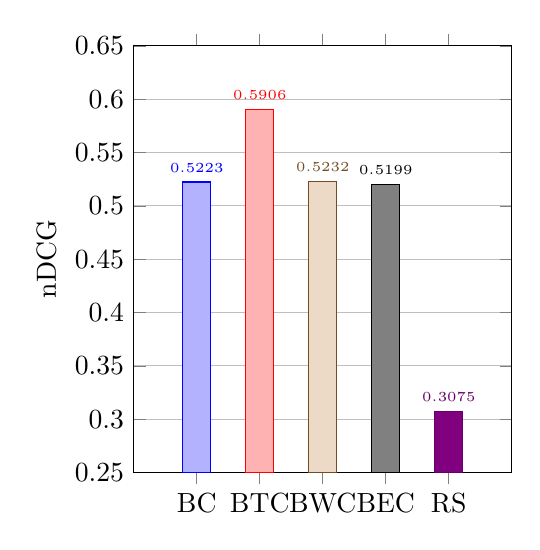
\begin{tikzpicture}
 \begin{axis}[
 	width=.75\textwidth,
 	height=7cm,
 	ybar =-10pt,
 	x = 0.80cm,
 	ymin=0.25, 	
 	ymax=0.65,
 	ytick = {0.25,0.30,...,0.70},
	enlarge x limits ={abs=.8cm},
	nodes near coords,
    every node near coord/.append style={font=\tiny,/pgf/number format/.cd,precision=4},
 	ylabel={nDCG},
	xtick={0,1,2,3,4},  % NEW BIT
	xticklabels={BC, BTC, BWC, BEC, RS},
	%legend style={at={(0.5,-0.1)},
	%anchor=north,legend columns=-1},
	ymajorgrids = true,]

		\addplot coordinates {(0,0.5223)};    
		\addplot coordinates {(1,0.5906)};    
		\addplot coordinates {(2,0.5232)};    
		\addplot coordinates {(3,0.5199)};    
		\addplot coordinates {(4,0.3075)};
        %\legend{BC, BTC, BWC, BEC, Random}
     \end{axis}
\end{tikzpicture}
\captionof{figure}{Groups with 20 users}
\label{fig:testresult20members}
\end{minipage}
\begin{minipage}{.46\textwidth}\centering
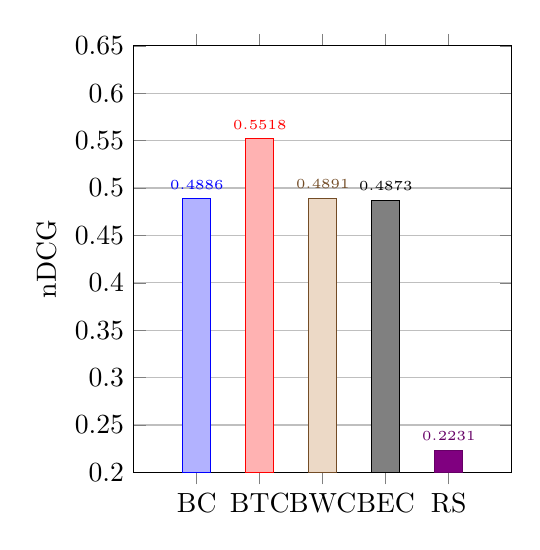
\begin{tikzpicture}
 \begin{axis}[
 	height=7cm,
 	ybar =-10pt,
 	x = 0.80cm,
 	ymin=0.20, 
 	ymax=0.65,	
 	ytick = {0.20,0.25,...,0.70},
	enlarge x limits ={abs=.8cm},
	nodes near coords,
    every node near coord/.append style={font=\tiny,/pgf/number format/.cd,precision=4},
 	ylabel={nDCG},
	xtick={0,1,2,3,4},  % NEW BIT
	xticklabels={BC, BTC, BWC, BEC, RS},
	%legend style={at={(0.5,-0.1)},
	%anchor=north,legend columns=-1},
	ymajorgrids = true,]

		\addplot coordinates {(0,0.4886)};    
		\addplot coordinates {(1,0.5518)};    
		\addplot coordinates {(2,0.4891)};    
		\addplot coordinates {(3,0.4873)};    
		\addplot coordinates {(4,0.2231)};
        %\legend{BC, BTC, BWC, BEC, Random}
     \end{axis}
\end{tikzpicture}
\captionof{figure}{Groups with 40 users}
\label{fig:testresult40members}
\end{minipage}
\end{figure}

\subsection{Influence of the Size of k} \label{sec:influenceofk}
While performing the satisfaction tests, an interesting observation regarding the size of $k$ was made. We tested BC and BTC with a few alternative $k$, and found that as $k$ increased from 10 to 20, there would be a drop in satisfaction. However at a $k$ of 50, this drop off had been more than made up for, with a satisfaction about 10\% points higher than the satisfaction at $k = 10$. Increasing k further to 100 also increases the satisfaction. These observations were found on tests performed on group sizes 16 and 40, other sizes were not tested.

During these prodding tests, it was discovered that there seemed to be a local maximum around a k of 10 or 11. These specific trends might be dependent on the dataset, as the only plausible explanation we could find, would be that the top-10 lists of each group holds comparatively more overlaps than the top-20 lists. For instance there might be 10 overlapping items in the top-10, while the top-20 only adds an extra 5 items with overlap, thus decreasing the percentage of items with an overlap in the set of items being evaluated upon. Similarly, top-50 might add a large number of new overlaps, increasing the final satisfaction, generally popular items could be located amongst items 21-50 in most users top-k lists.

\subsection{Evaluation of Results} \label{sec:evaluationofresults}
Based on the results presented in Section \ref{sec:satisfationevaluation} it seems that BTC performs remarkably well on group sizes of more than 8. If the results for group sizes 20 and 40 are any indication, then BTC is about 13\% better at satisfying a large group, when giving them 10 ordered items. On a group size of 4, BTC performs similarly to the other methods however slightly worse. Therefore, BTC should be used over BC when dealing with groups of size 8 or more.

As indicated by the findings presented in Section \ref{sec:influenceofk}, which value of $k$ that is used has little influence on which aggregation that performs best. However it has a large effect on how much satisfaction that is achieved overall. Ideally, for the MovieLens dataset, $k$ should be 10 if the recommender should return a small number of items, otherwise it would be best to have it at more than 50. Whether this is generally applicable remains to be seen.

These results are a reflection of the evaluation performed on the MovieLens dataset, therefore, as mentioned in Section \ref{sec:limitsetup}, the results should be tested on other datasets before anything can be concluded about the general application of the algorithms. That being said BTC shows promise and further study of the approach would be in order. 



%  BTC
% k = 20   s = 12   0,5666
% k = 10   s = 12   0,5934
% k = 8    s = 12   0,6427
% k = 5    s = 12   0,5857
% k = 8    s = 40   0,5288
% k = 10   s = 40   0,5518
% k = 11   s = 40   0,5531
% k = 12   s = 40   0,5501
% k = 20   s = 40   0,5287
% k = 50   s = 40   0,5970
% k = 100  s = 40   0,6857

% k = 11   s = 16   0,5767
% k = 20   s = 16   0,5534
% k = 50   s = 16   0,6276

% Random
% k = 20   s = 16   0,3690
% k = 50   s = 16   0,37

% Borda
% k = 20   s = 12   0,5695
% k = 8    s = 12   0,5455
% k = 20   s = 40   0,5213
% k = 50   s = 40   0,5964
% k = 100  s = 40   0,6853



% k = 10:
% s = 4     0,6394
% s = 8     0,6044
% s = 12    0,5934
% s = 16    0,5939
% s = 20    0,5906
% s = 40    0,5518